\documentclass[12pt,a4paper]{article}
\usepackage[utf8]{inputenc}
\usepackage{graphicx}
\usepackage{hyperref}
\usepackage{listings}
\usepackage{xcolor}
\usepackage{geometry}
\usepackage{float}

\geometry{margin=2.5cm}

\title{Übung 4 - Android}
\author{Student: Philip Magnus}
\date{}

\begin{document}

\maketitle


\section{Lab + App Network Traffic Inspection/Interception Setup}

The steps in this writeup were performed on a Windows 11 (x64) system.

\subsection{Lab environment using a Android device and/or emulator (e.g. Android Emulator)}

The following steps describe the setup of the needed lab environment. For ease of use I choose to setup an android emulator via \texttt{Android Studio}.

First \texttt{Android Studio} was installed via the JetBrains Toolbox.

\begin{figure}[H]
\centering
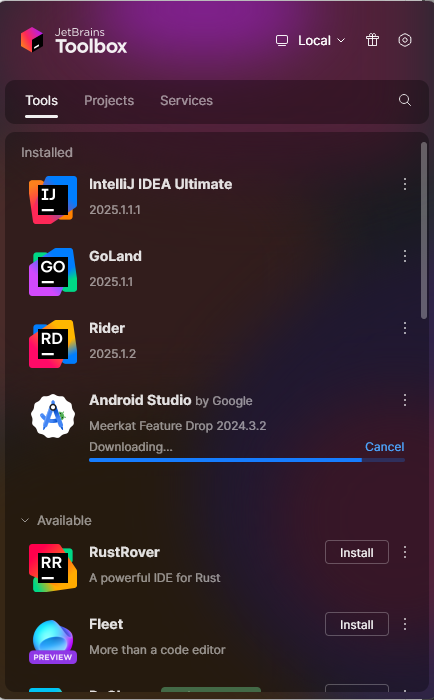
\includegraphics[width=.4\textwidth]{./screenshots/install_android_studio.png}
\caption{Install Android Studio}
\end{figure}

In \texttt{Android Studio} we open the \texttt{Virtual Device Manager} and open the setup wizard for creating a new virtual device.

\begin{figure}[H]
\centering
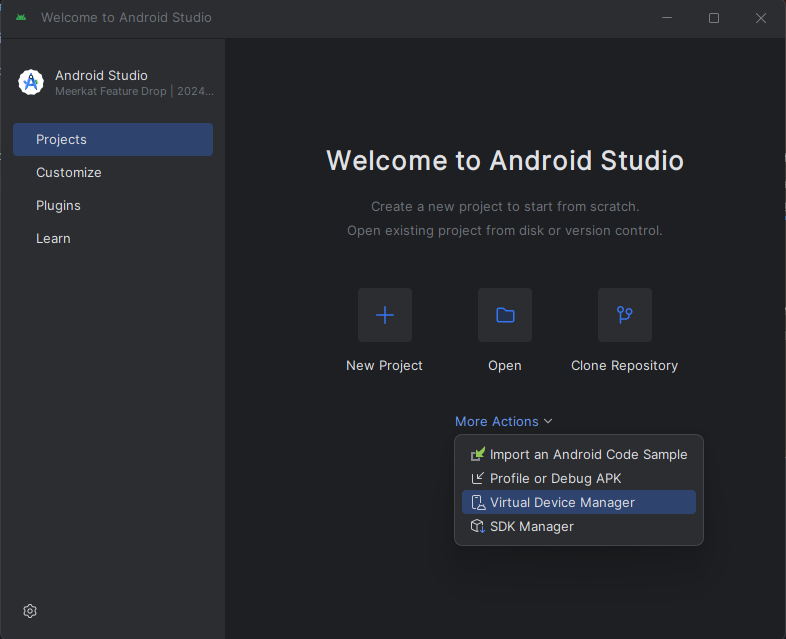
\includegraphics[width=0.8\textwidth]{./screenshots/android_virtual_dev_manager.png}
\caption{VirtualDev Manager}
\end{figure}

In the device setup I chose to use the Google APIs for an easier setup of \texttt{httptoolkit} later on. Android 15 was chosen as the Android version to install on the virtual device.

\begin{figure}[H]
\centering
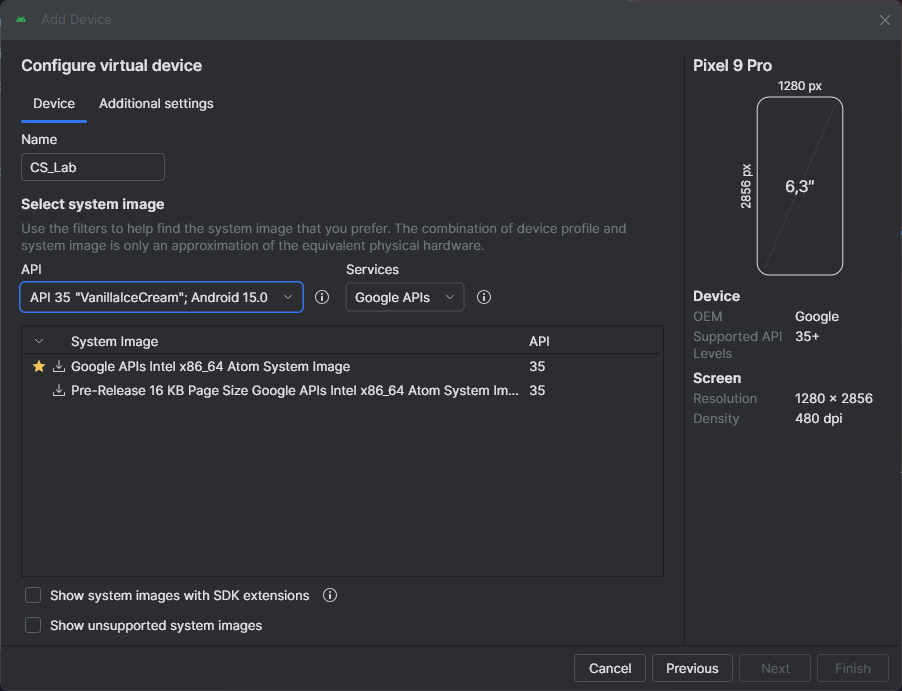
\includegraphics[width=0.8\textwidth]{./screenshots/dev_apis.png}
\caption{Device APIs}
\end{figure}

As the system image \texttt{Google APIs Intel x86\_64 Atom System Image} was used. For our scenario there is no need for the pre-relese image.
With clicking the \texttt{Finish} button the installation of the device started.

\begin{figure}[H]
\centering
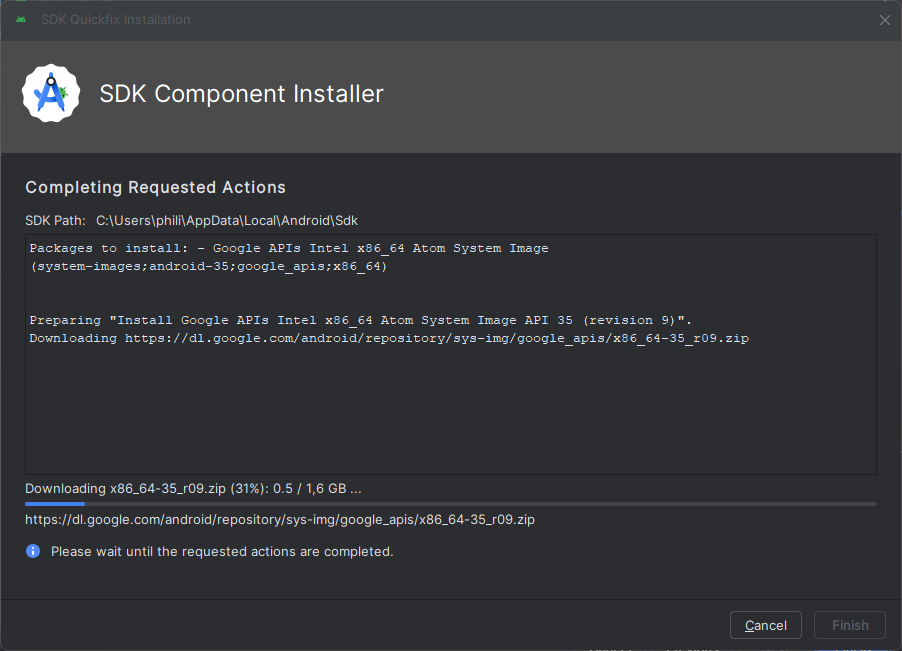
\includegraphics[width=0.8\textwidth]{./screenshots/android_em_install.png}
\caption{Emulator Install}
\end{figure}

After the installation the "fresh" virtual device can be started simply via the virtual device manager. After starting the device I was greeted by an almost empty home screen.

\begin{figure}[H]
\centering
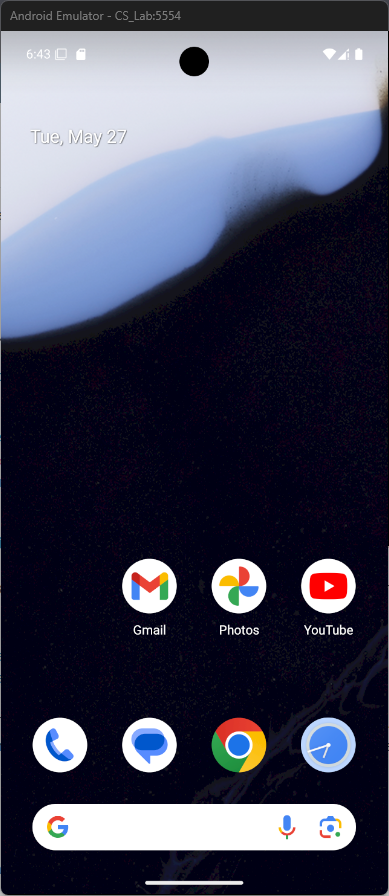
\includegraphics[width=.25\textwidth]{./screenshots/fresh_virtual_dev.png}
\caption{Fresh device emulator}
\end{figure}

\clearpage

\subsection{Choose an arbitrary app with HTTP(S) backend communication}

As the target app I chose the \texttt{ORF.at News} app. The app is currently in version 1.99.37 and needs at least Android 5, or the \texttt{Lollipop, API 21}, installed.

\begin{figure}[H]
\centering
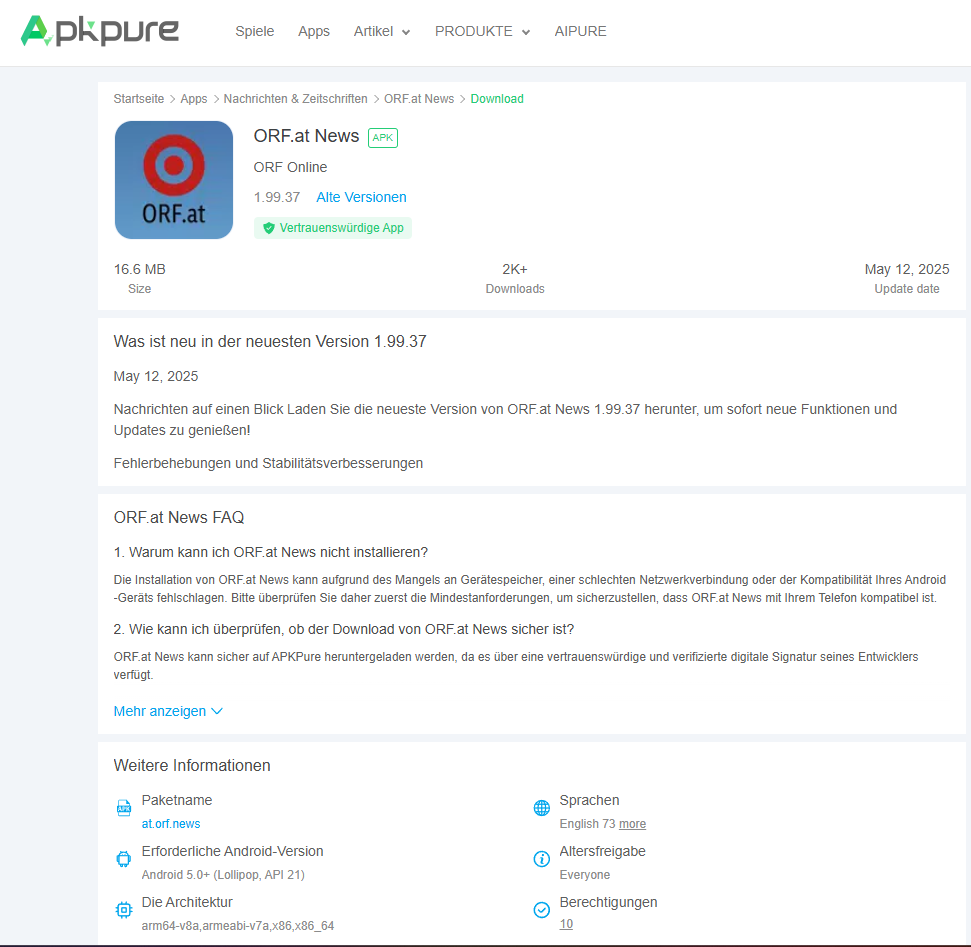
\includegraphics[width=0.8\textwidth]{./screenshots/apkpure.png}
\caption{ApkPure}
\end{figure}

Installing the app is very simple and can be achieved by dragging the app onto the virtual device. The app is then automatically installed and can be used from there.

\begin{figure}[H]
\centering
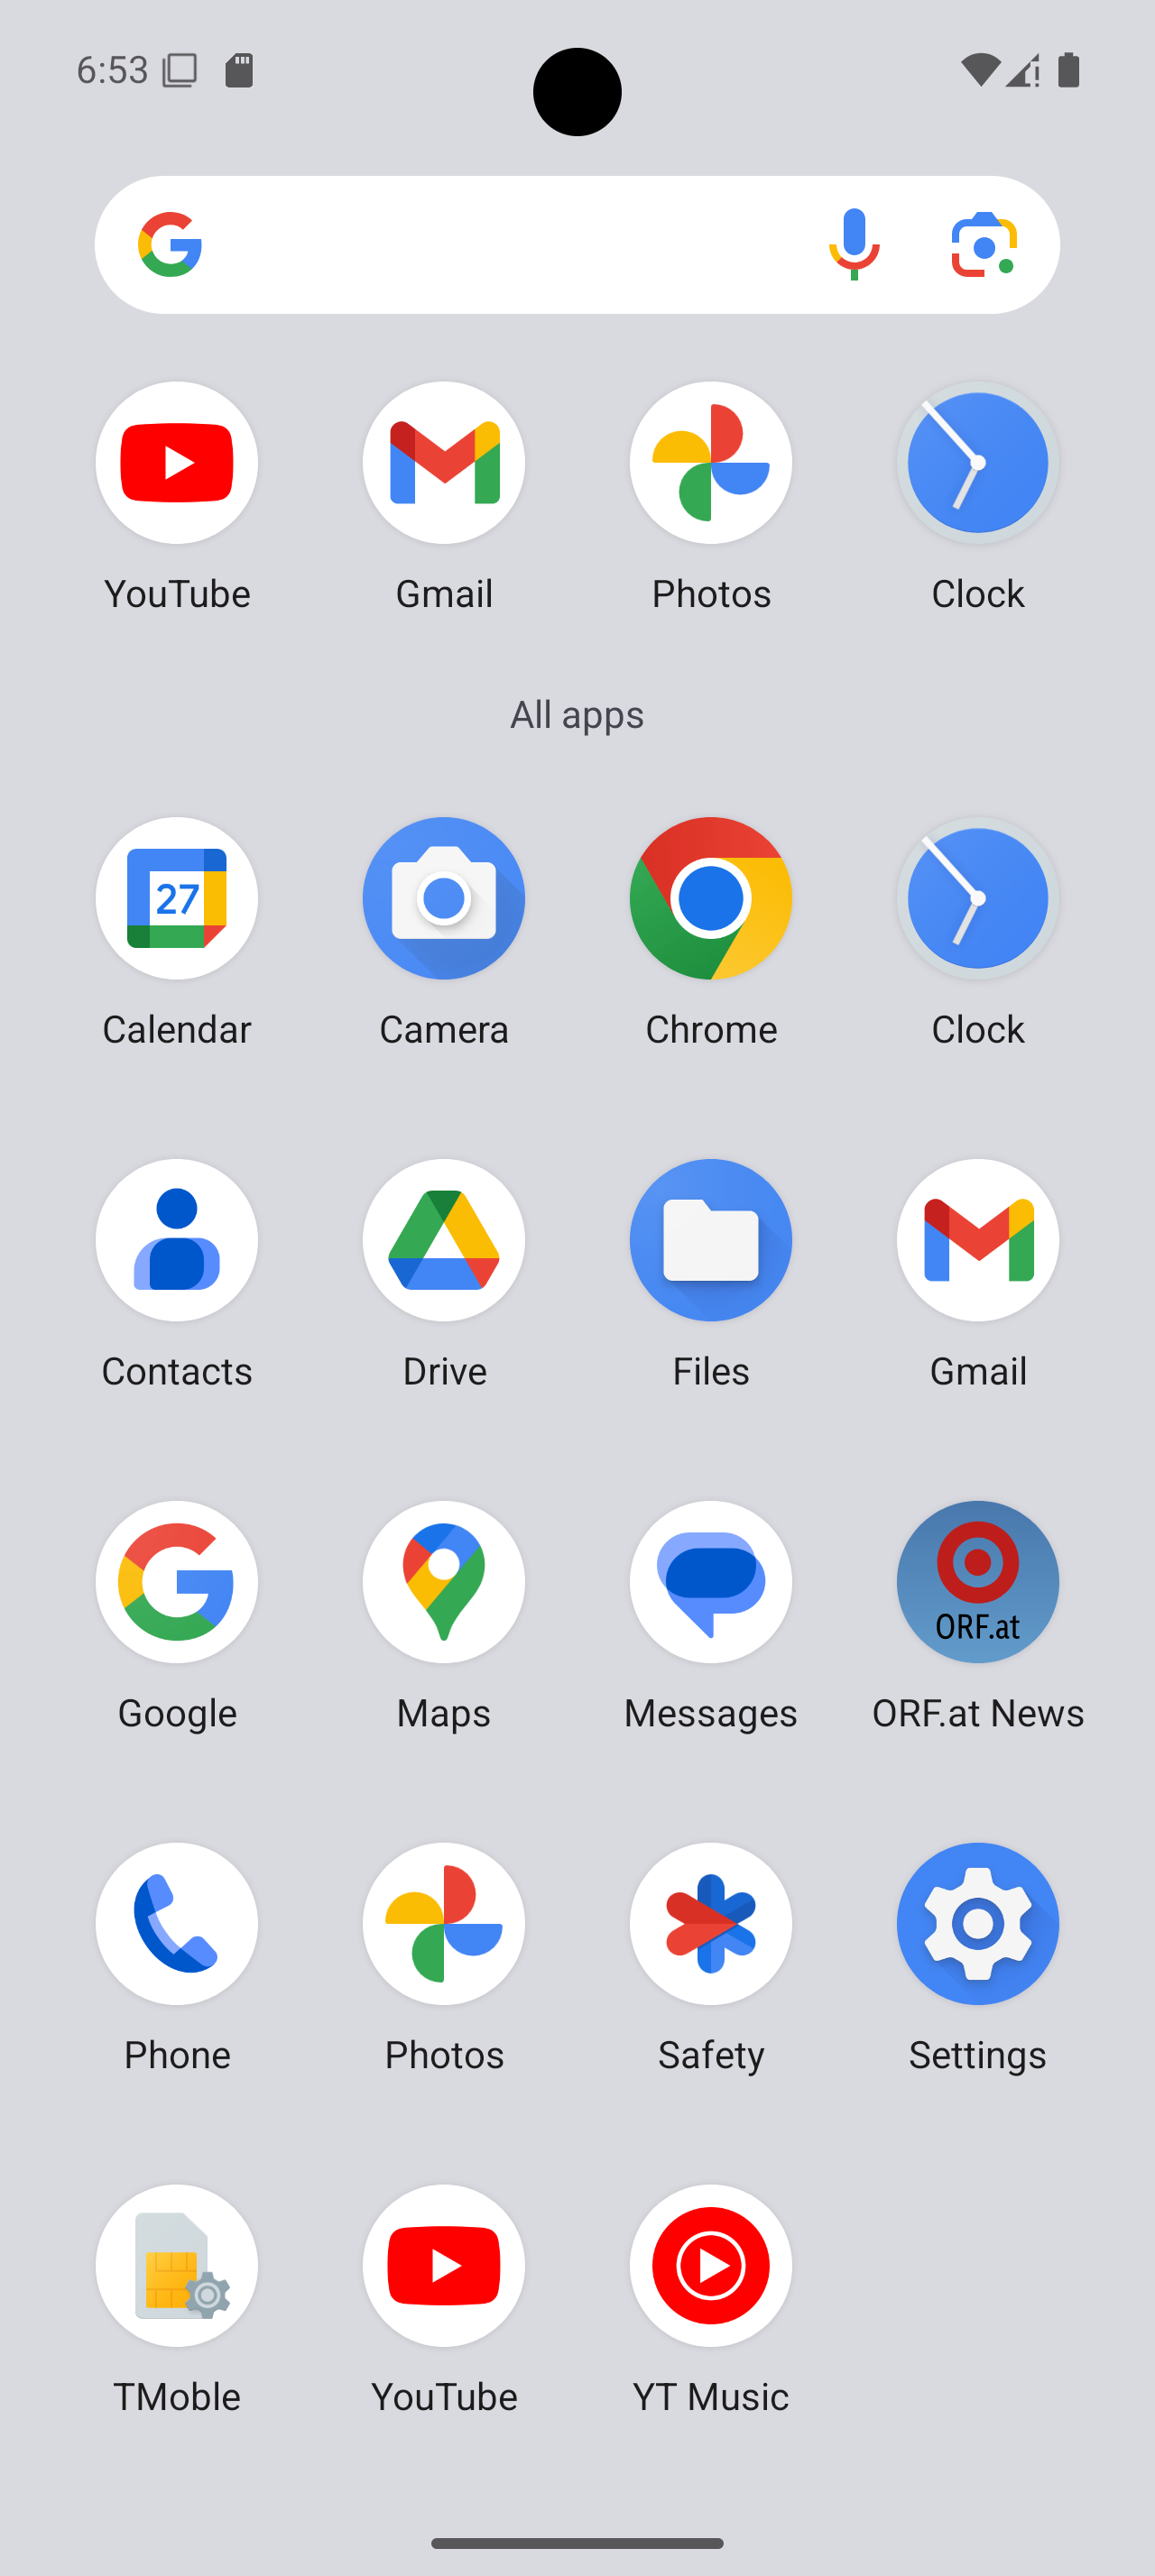
\includegraphics[width=.25\textwidth]{./screenshots/orfat_app.png}
\caption{ORF.at}
\end{figure}

Next I installed \texttt{httptoolkit}. After the installation under intercept I chose the \texttt{Android device via ADB} setup. The setup completes pretty much automatically and lets me sniff any http/https traffic on the device.

\begin{figure}[H]
\centering
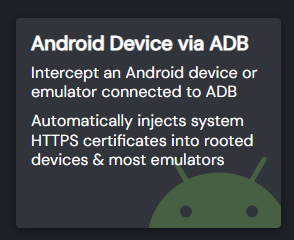
\includegraphics[width=0.6\textwidth]{./screenshots/http_toolkit_adb.png}
\caption{via ADB}
\end{figure}

During the setup I only needed to approve \texttt{httptoolkit}'s access only once on the virtual device.

\begin{figure}[H]
\centering
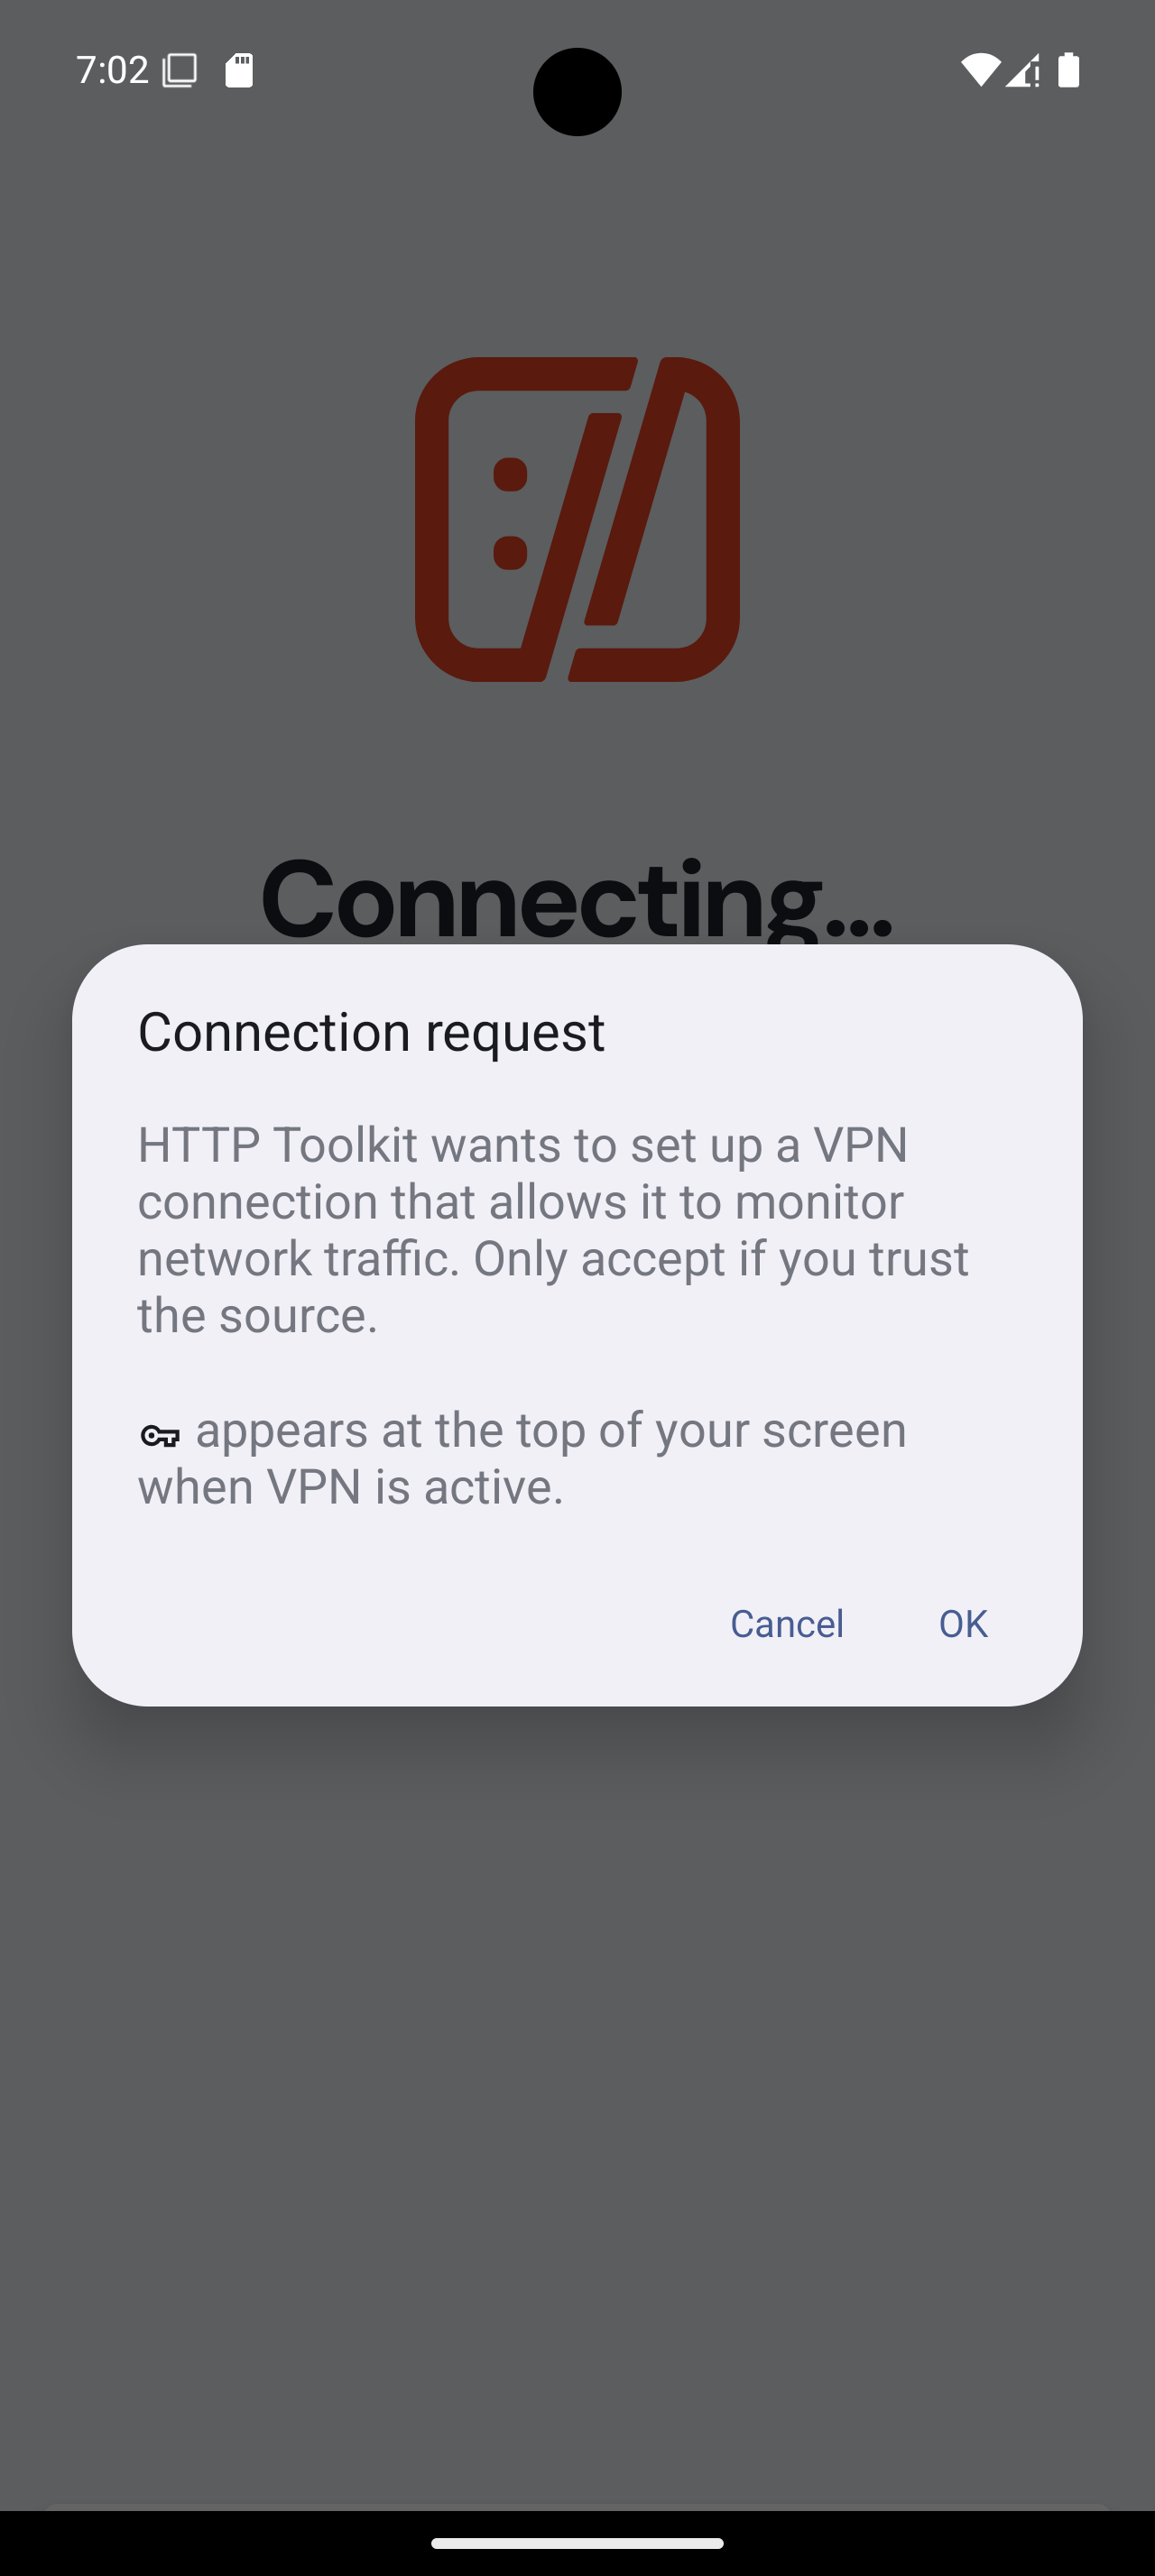
\includegraphics[width=.25\textwidth]{./screenshots/approve_toolkit.png}
\caption{approve toolkit}
\end{figure}

After the approval I was able to see all traffic on the device. For example opening a random article in the \texttt{ORF.at News} app resulted in quiet some observable http traffic.

\begin{figure}[H]
\centering

\includegraphics[width=.25\textwidth]{./screenshots/article_app.png}
\caption{article in app}
\end{figure}

\begin{figure}[H]
\centering
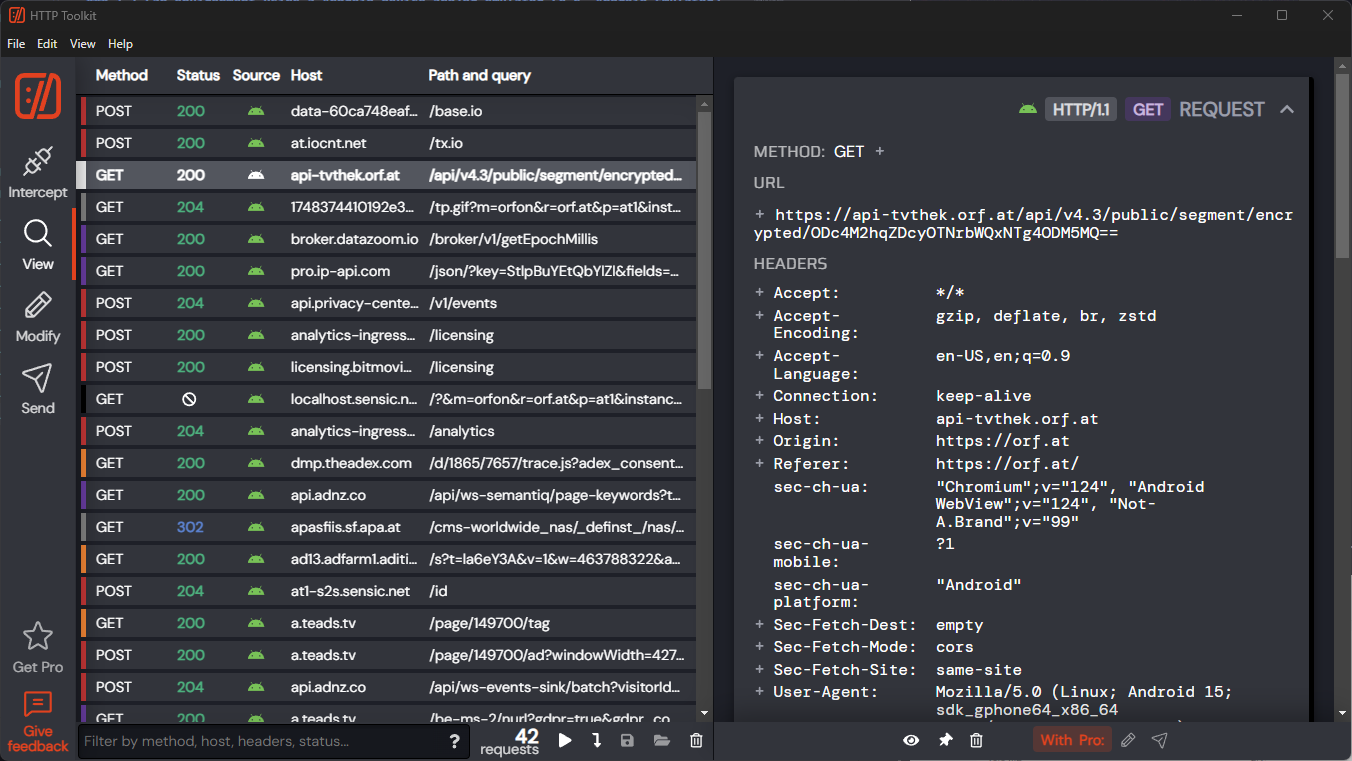
\includegraphics[width=0.8\textwidth]{./screenshots/httptoolkit.png}
\caption{http toolkit traffic}
\end{figure}

\section{Perform Static and Dynamic Analysis}

The following steps describe the static and dynamic analysis of the app. The goal is to find out how the app communicates with the backend and what data is sent/received.

\subsection{Static: inspect the source code to analyze the HTTP(S) implementation}

\subsubsection{Decompile the application, e.g. using Bytecode Viewer, APK Editor Studio, apktool, JADX, Ghidra, etc.}

First I downloaded the \texttt{JADX} software from the official Github repository. 
After extracting the downloaded archive, \texttt{JADX} can be started through the included .exe file.

\begin{figure}[H]
\centering
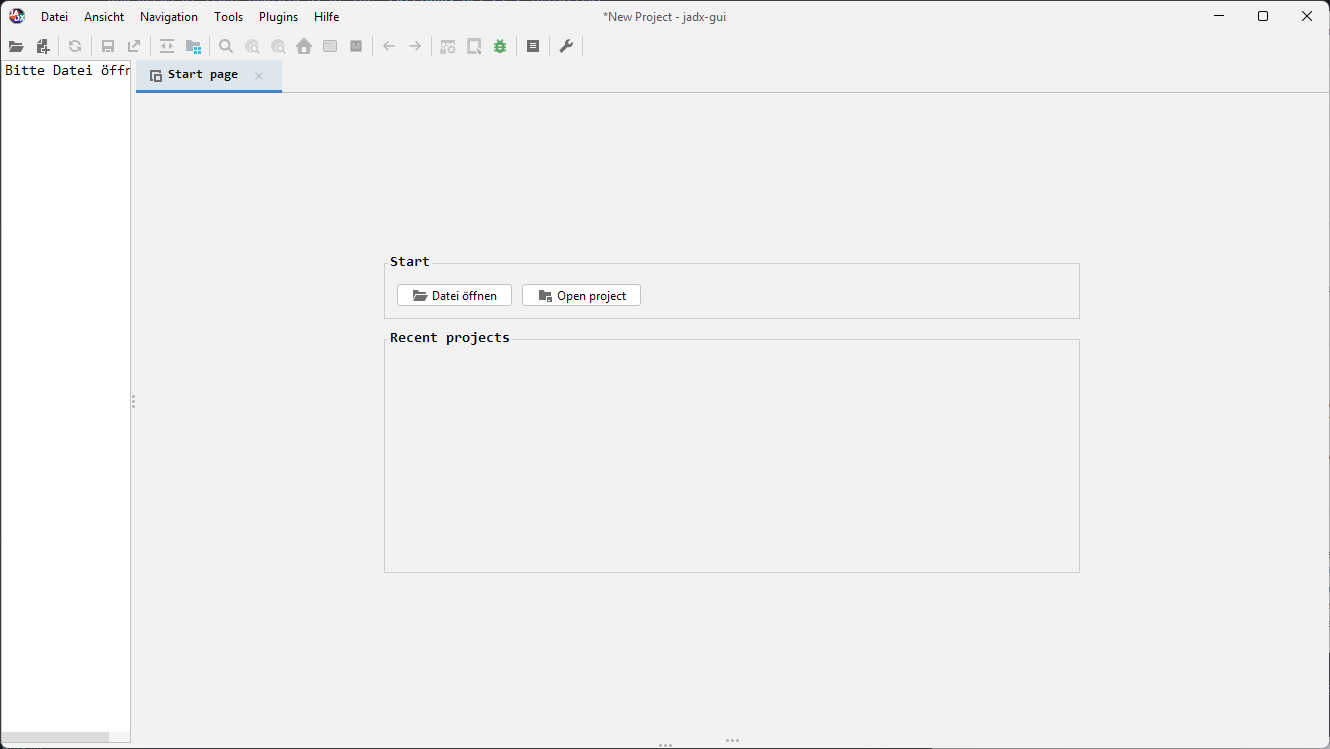
\includegraphics[width=0.8\textwidth]{./screenshots/jadx_initial.png}
\caption{JADX start}
\end{figure}

By clicking the \texttt{Open File} I was able to select the file to decompile.

\begin{figure}[H]
\centering
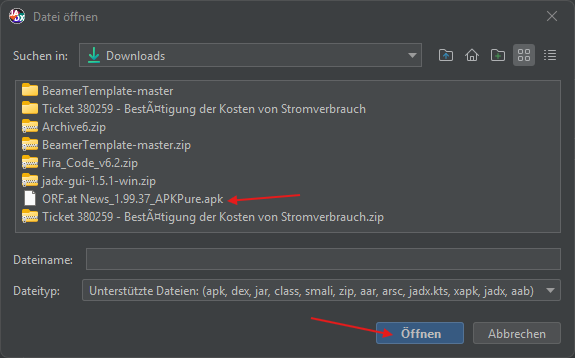
\includegraphics[width=0.8\textwidth]{./screenshots/opening_apk.png}
\caption{Opening APK}
\end{figure}

After opening the file, \texttt{JADX} started decompiling the app. The decompilation took a few seconds and afterwards I was able to browse through the code of the app.

\begin{figure}[H]
\centering
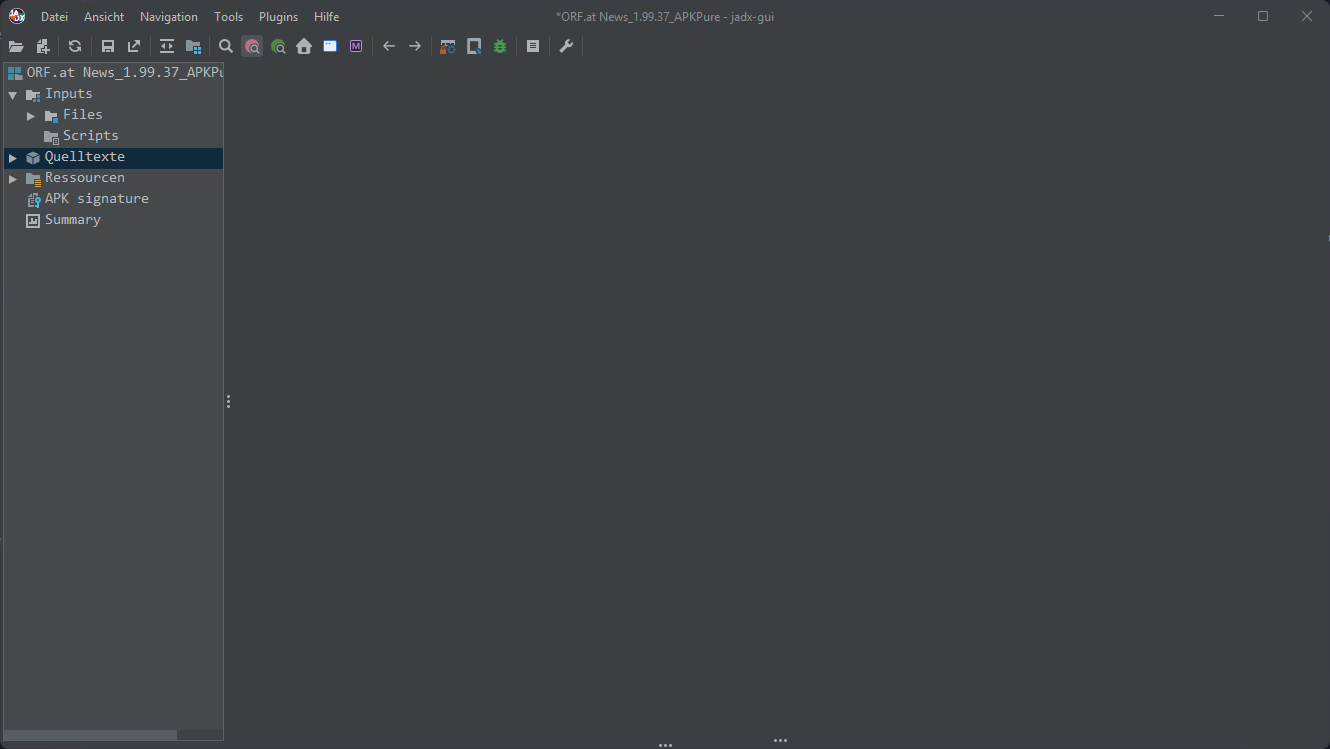
\includegraphics[width=0.8\textwidth]{./screenshots/jadx_decompiled.png}
\caption{Decompiled code}
\end{figure}


\subsubsection{How is HTTP(S) is implemented?}

In the decompiled code are several hints on how the app communicates with the backend. The app uses the \texttt{Retrofit2} and \texttt{OkHttp} library to handle HTTP requests.
The app seems to use \texttt{Retrofit2} for making https calls. \texttt{Retrofit2} is a type-safe HTTP client which in turn implements the \texttt{OkHttp} library to handle the actual network requests.

\begin{figure}[H]
\centering
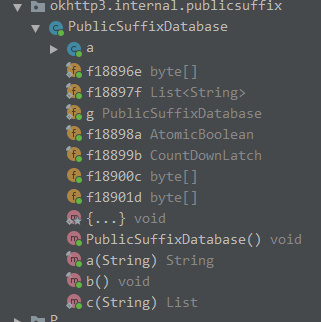
\includegraphics[width=0.8\textwidth]{./screenshots/okhttp.png}
\caption{OkHttp}
\end{figure}

\begin{figure}[H]
\centering
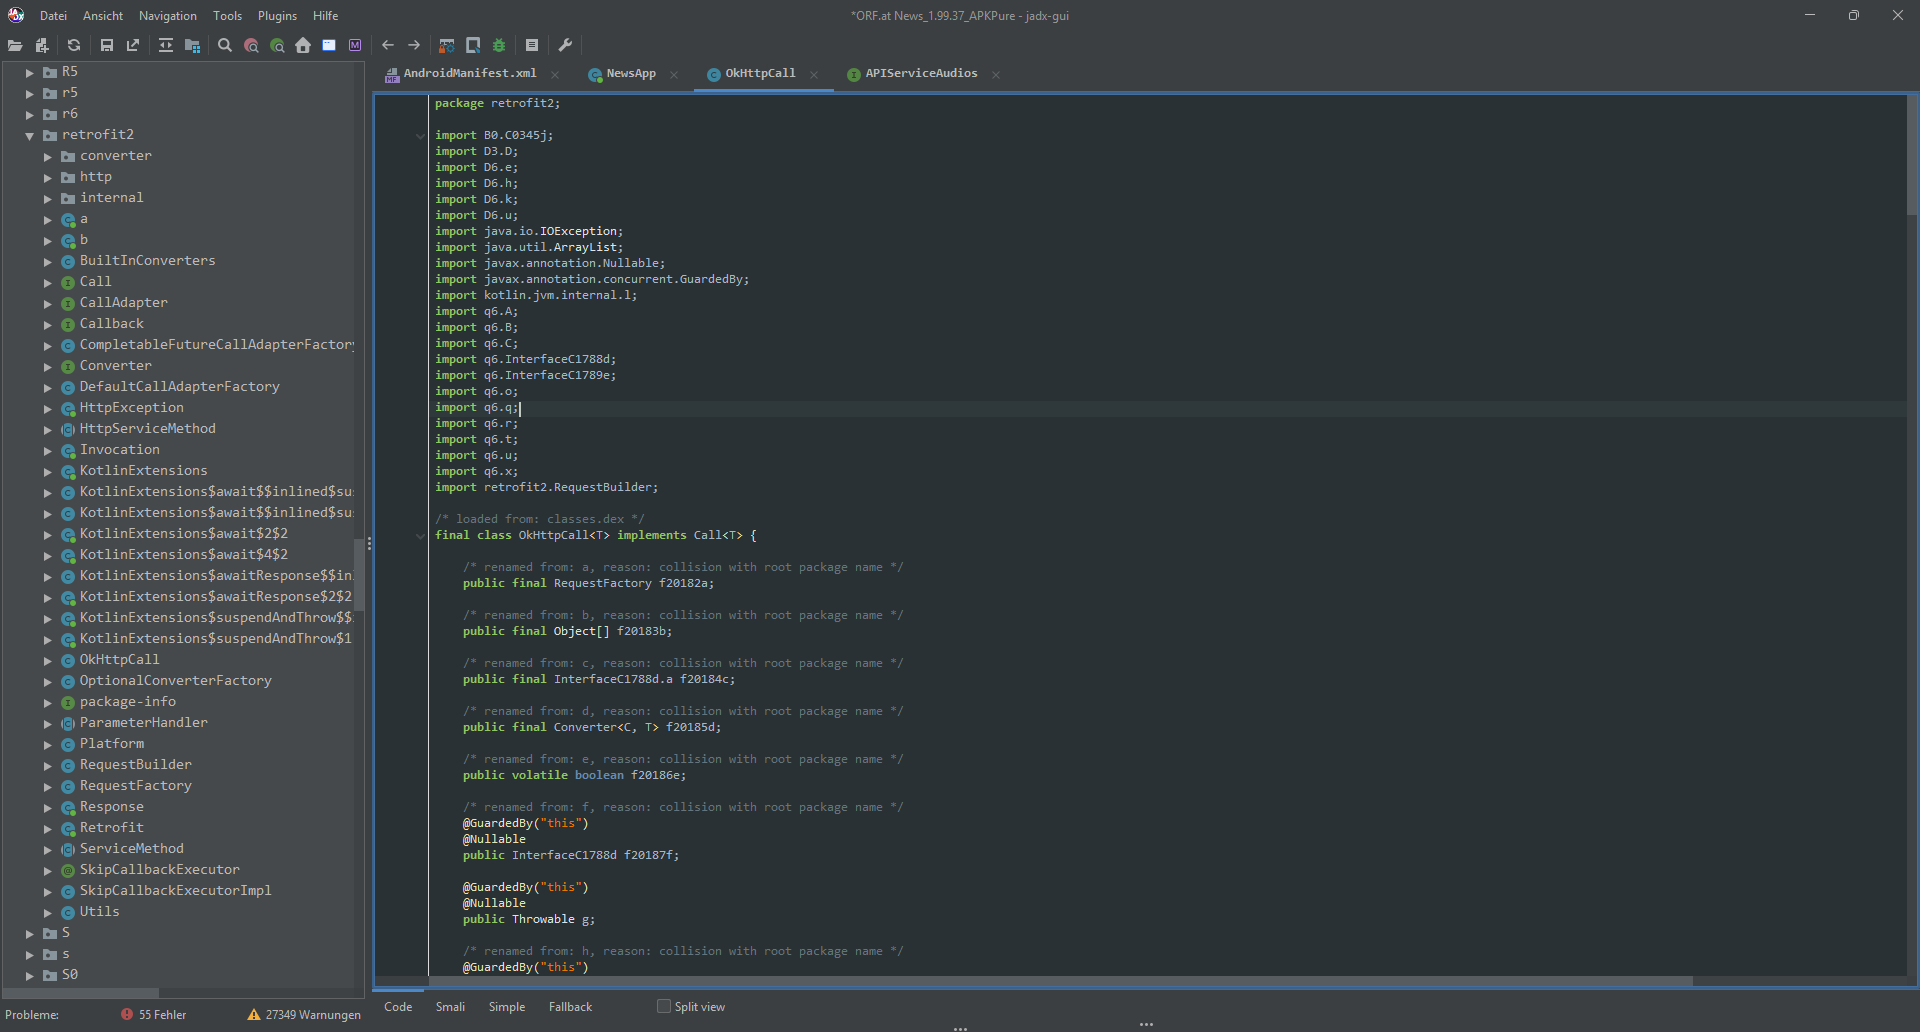
\includegraphics[width=0.8\textwidth]{./screenshots/retrofit_dec.png}
\caption{Retrofit2 decompilation}
\end{figure}

\begin{figure}[H]
\centering
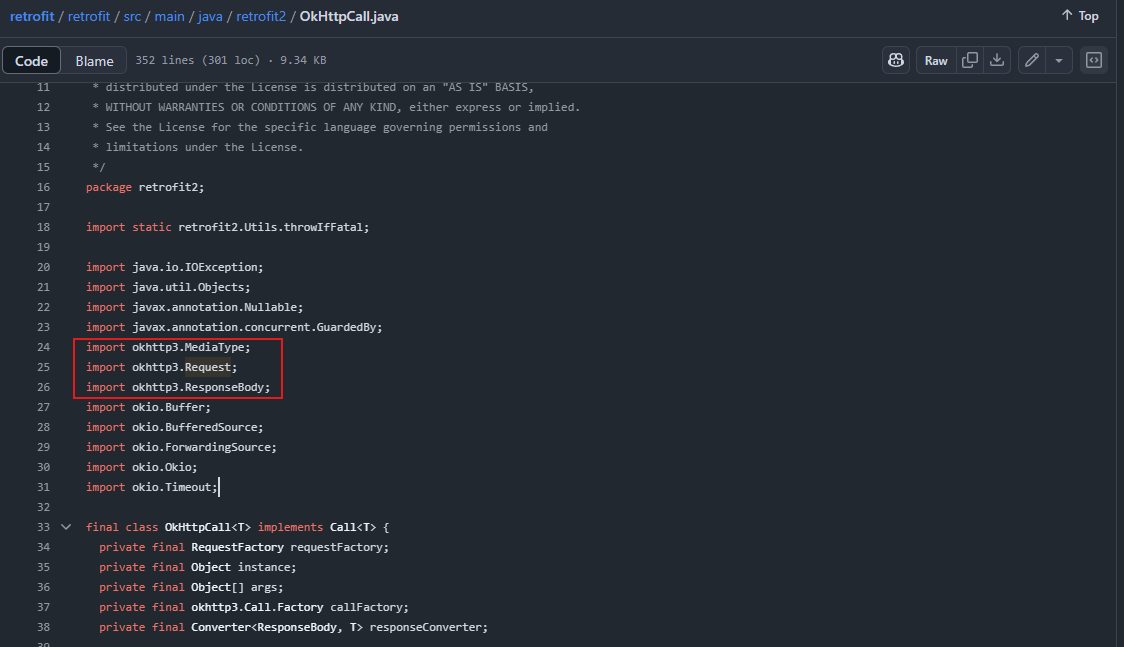
\includegraphics[width=0.8\textwidth]{./screenshots/retrofit_okhttp.png}
\caption{Retrofit2 OkHttp implementation}
\end{figure}

The app does not only use \texttt{Retrofit2} and \texttt{OkHttp} for network requests, it also uses \texttt{android-async-http} from \texttt{loopj} for some network requests.
\texttt{android-async-http} in turn implements the \texttt{httpclient-android} library to handle the actual network requests. This library is a port of the Apache HttpClient to Android.

The following code snippet shows the usage of \texttt{android-async-http} in the decompiled code:

\begin{figure}[H]
\centering
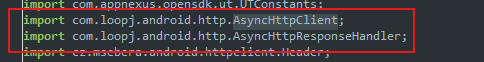
\includegraphics[width=0.8\textwidth]{./screenshots/asyncHttpClient.png}
\caption{AsyncHttpClient}
\end{figure}

As we can see in the code snippet, the \texttt{httpclient-android} library is imported and used to make network requests.

\begin{figure}[H]
\centering
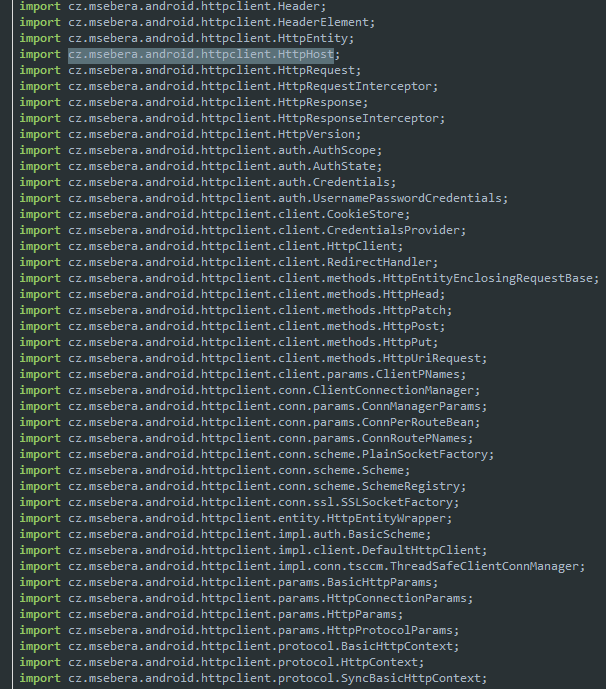
\includegraphics[width=0.8\textwidth]{./screenshots/msebera_http.png}
\caption{httpclient-android import}
\end{figure}


\subsubsection{Which TLS versions and cipher suites are supported?}

Accordrding to the official \texttt{OkHttp} documentation "OkHttp supports modern TLS features (TLS 1.3, ALPN, certificate pinning)".
Given that the app uses \texttt{OkHttp} to handle the network requests, it can be assumed that the app supports TLS 1.3 and the cipher suites provided by \texttt{OkHttp}.

For more information on the supported cipher suites, the official \href{https://github.com/square/okhttp}{Github repository} can be consulted.

For requests made with \texttt{android-async-http} the supported TLS versions and cipher suites depend on the underlying \texttt{httpclient-android} library. In the implementation I could not find any
specific supported TLS version but the library uses the Cypher Suites provided by the Android system.

\begin{figure}[H]
\centering
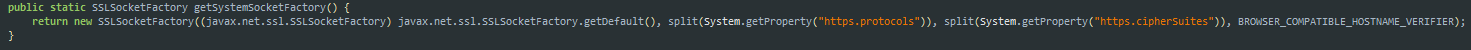
\includegraphics[width=0.8\textwidth]{./screenshots/system_cyphersuites.png}
\caption{System Cipher Suites}
\end{figure}

\subsubsection{Is a Network Security Configuration (NSC) used? Is Certificate Pinning implemented?}

Neither a Network Security Configuration (NSC) nor Certificate Pinning was found in the decompiled code. The app seems to rely on the default behavior of \texttt{OkHttp} and \texttt{Retrofit2} for handling SSL/TLS connections.

I came to this conclusion because the necessary configurateion files for NSC were not present in the decompiled code. The quickest way to check for the presence of a NSC is to look for a file named \texttt{network\_security\_config.xml} in the \texttt{res/xml} directory of the decompiled app.

\begin{figure}[H]
\centering
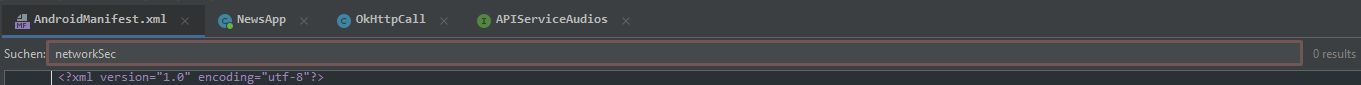
\includegraphics[width=0.8\textwidth]{./screenshots/no_nsc.png}
\caption{No NSC found in AndroidManifest.xml}
\end{figure}

The app was written with an API level of 21 in mind, if I am not mistaken this means that the app does not support a Network Security Configuration (NSC), as NSC was introduced in API level 23.

\subsection{Dynamic: inspect generated network traffic \& analyze communication to backend servers}

\subsubsection{Is any sensitive information sent to the backend server?}

After generating some traffic within the app and anylzing it with \texttt{httptoolkit}, I was not able to find any sensitive information being sent to the backend server. 
The app seems to only send the necessary data for fetching news articles and other related content.

\begin{figure}[H]
\centering
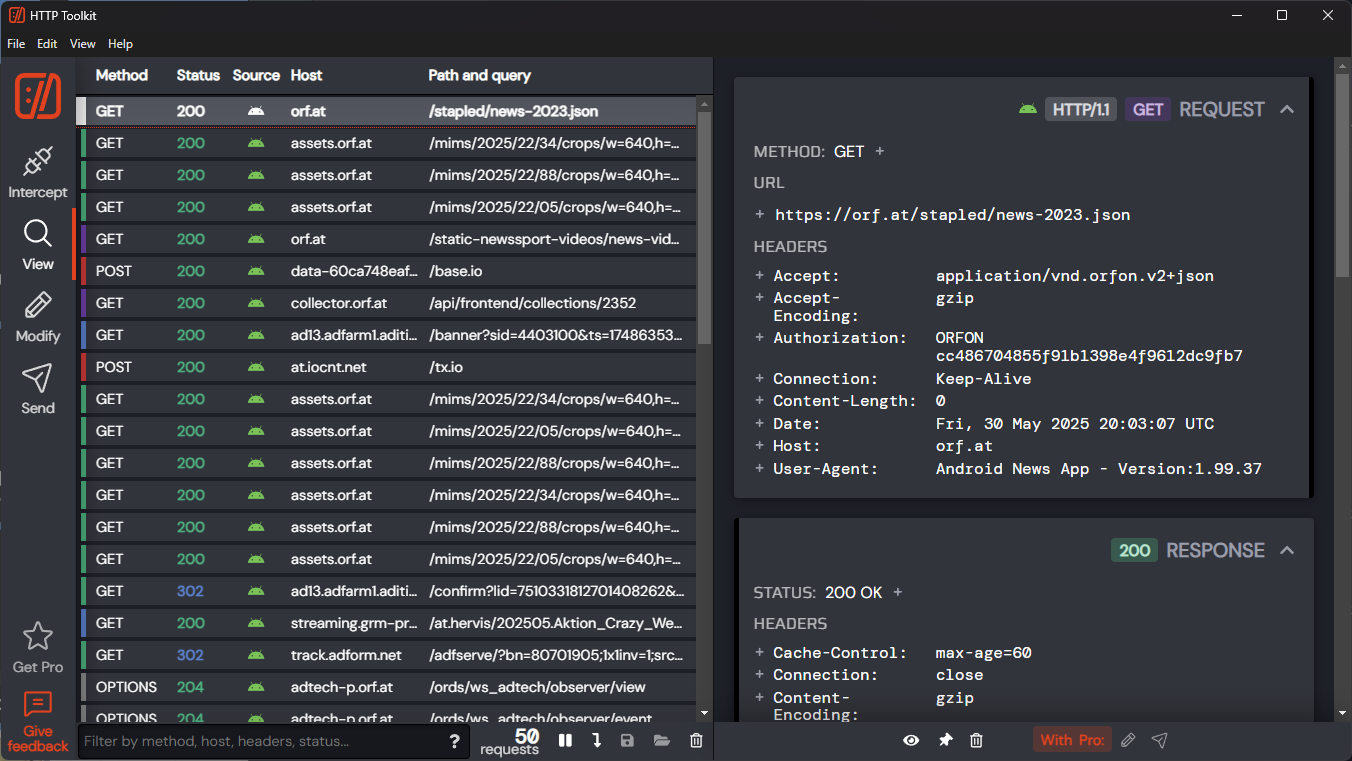
\includegraphics[width=0.8\textwidth]{./screenshots/Traffic_analyzation.png}
\caption{Traffic analyzation}
\end{figure}

\subsubsection{Does the app collect analytics?}

The app does seem to collect some analytics data, but it is not clear what exactly is being collected. The app does not seem to collect any sensitive information, but it does send some data to the backend server for analytics purposes.
By looking at the traffic with some educated guessing, I assume the app collects some analytics data for serving advertisements to the user.

\begin{figure}[H]
\centering
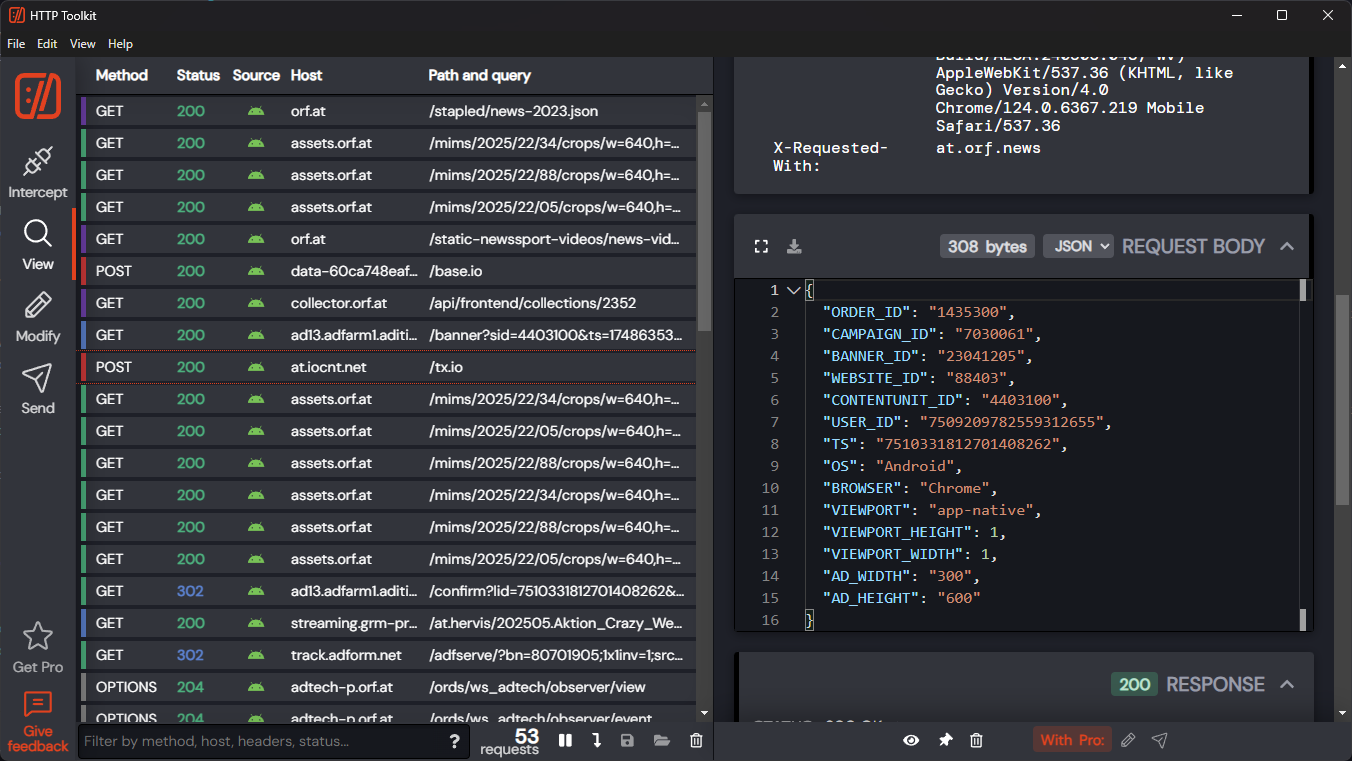
\includegraphics[width=0.8\textwidth]{./screenshots/ad_tracking.png}
\caption{Ad Tracking}
\end{figure}

Some other minor analytics like the android version are send to the backend probably to ensure compatibility with the app.

\begin{figure}[H]
\centering
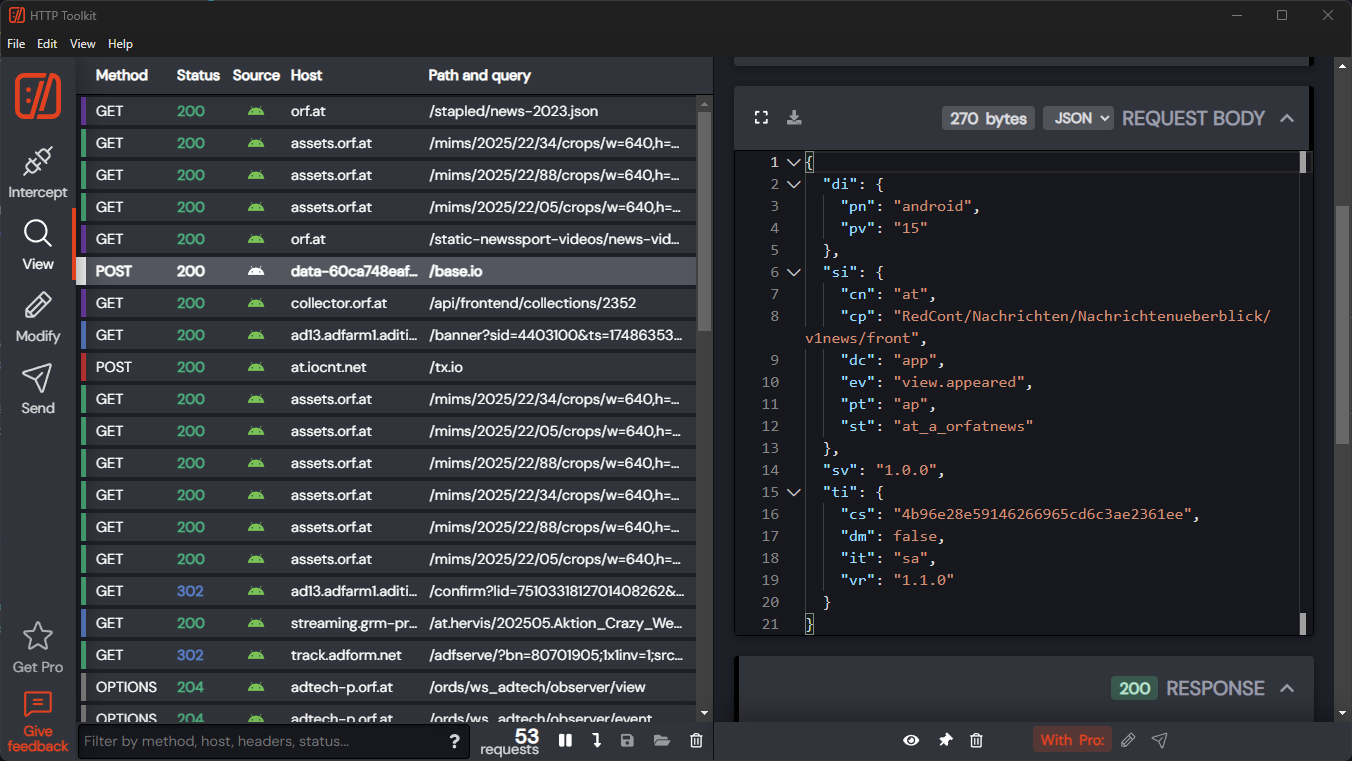
\includegraphics[width=0.8\textwidth]{./screenshots/minor_tracking.png}
\caption{Minor Tracking}
\end{figure}

In the decompiled code I found some configuration files hinting at a \texttt{Firebase} integration. 
The app seems to send some analytics data to \texttt{Firebase} for further processing, although I was not able to see any live traffic confirming this theory.

\begin{figure}[H]
\centering
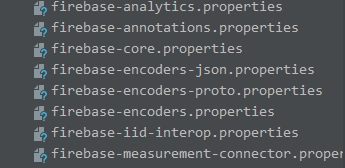
\includegraphics[width=0.8\textwidth]{./screenshots/Firebase_integration.png}
\caption{Firebase integration}
\end{figure}
 
\subsubsection{Are there any hard-coded secrets in the app (i.e. authorization tokens, etc.)?}

One secrets seem to be hard-coded in the app. The app does use a hardcoded API auth-token for accessing the backend server.

\begin{figure}[H]
\centering
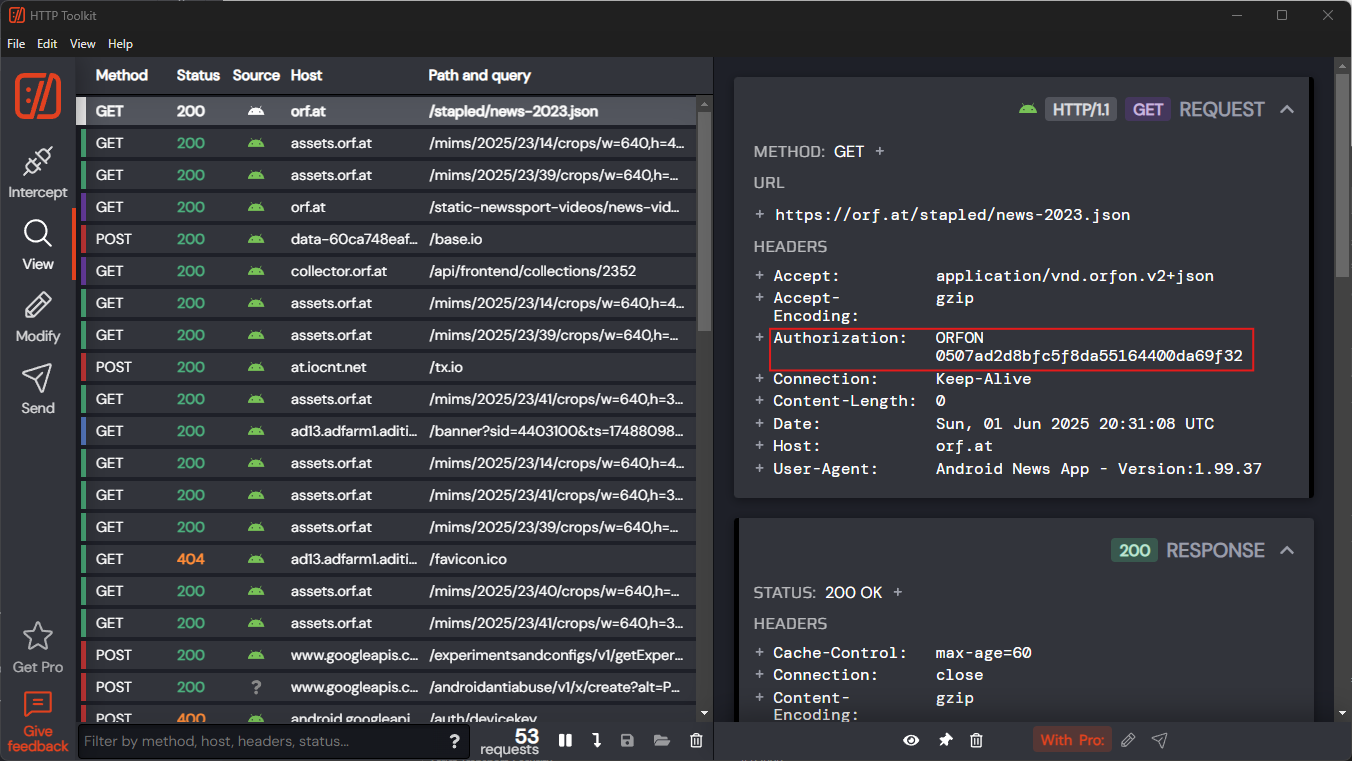
\includegraphics[width=0.8\textwidth]{./screenshots/Auth_header.png}
\caption{Auth Header}
\end{figure}

The following code snippet shows the usage of the hardcoded API auth-token in the decompiled code:

\begin{figure}[H]
\centering
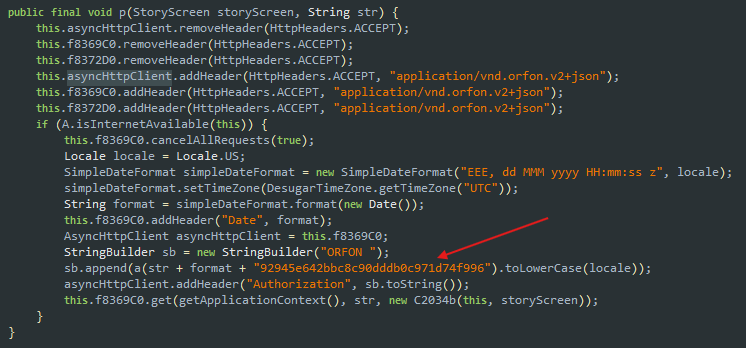
\includegraphics[width=0.8\textwidth]{./screenshots/hardcoded_token.png}
\caption{Hardcoded Auth Token}
\end{figure}

Beyond that I was not able to find any hard-coded secrets in the app. The app seems to rely on the backend server for further authentication and does not store any sensitive information locally.

\subsubsection{Any other interesting findings in the communication (e.g. in regard to OWASP Mobile Top 10)?}

Regarding the OWASP Mobile Top 10, I did not find any major issues in the app.
The most interesting part would concern the apps supply chain security. This would fall under \texttt{M2: Inadequate Supply Chain Security}. Some of the libraries in used in the app are rather old and 
have not been updated in quite some time, sometimes years. This could lead to potential security issues in the future, as the libraries might not be maintained anymore and could contain vulnerabilities.

If those packages have been downloaded by another library or were purposefully integrated into the app is not clear.

\begin{figure}[H]
\centering
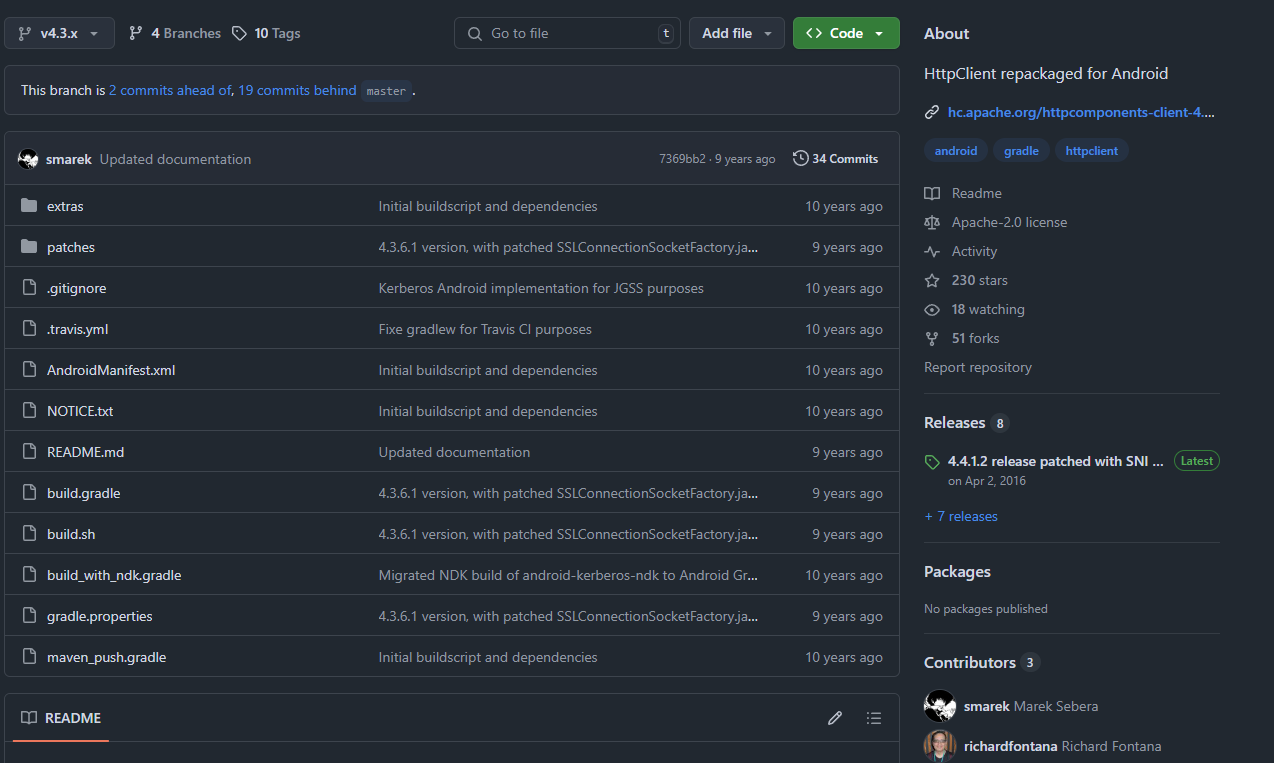
\includegraphics[width=0.8\textwidth]{./screenshots/old_repository.png}
\caption{Unmaintained repository - httpclient}
\end{figure}

\section{Conclusion}

In conclusion, the app does not seem to have any major security issues. The app uses \texttt{OkHttp} and \texttt{Retrofit2} for handling network requests, which are both well-known libraries in the Android ecosystem. 
The app does not use a Network Security Configuration (NSC) or Certificate Pinning, also it does not seem to send any sensitive information to the backend server. It should be noted that NSC was introduced in API level 23, which is higher than the minimum API level of the app (21).
They also should consider switching to libraries that are actively maintained.

\end{document}